\chapter{Einführung}
In Anbetracht der Tatsache, dass neuronale Netzwerke in Zukunft eine grössere Rolle spielen, wird in diesem Dokument
das Ziel verfolgt, die Mathematik dahinter verständlich zu erklären. Es werden einige Vorkenntnisse im Bereich der neuronalen Netze
vorausgesetzt. Diese werden in diesem Dokument nicht näher erläutert. Für Leser, welche sich im Gebiet der
Differentialrechnung und Optimierung noch nicht so gut auskennen, sei hier an dieser Stelle geraten, den Anhang zu lesen.
\\

Grundsätzlich bildet ein neuronales Netz einen gegebenen Input auf einen Output ab, ist also nichts weiteres als
eine Funktion. Diese Funktion wiederum ist mehrdimensional, hat also mehrere Input-Variablen und bildet diese wiederum
auf einen mehrdimensionalen Output um $f: \mathbb{R}^m \rightarrow \mathbb{R}^n$. Die Input-Variablen sind die Gewichte, die Output-Werte
die Klassen\footnote{Sollen z.B. in einem Bild Hunde und Katzen erkannt werden, so gibt es zwei Klassen \glqq Hund\grqq{} und \glqq Katze\grqq.
In dem Fall ist die Output-Dimension zweidimensional.}. Grundsätzlich werden nun die Gewichte dieses neuronalen Netzes so trainiert, dass eine gewählte Fehlerfunktion
möglichst minimiert wird. Man befindet sich hier im Bereich der Optimierung. In Abbildung \ref{fig:05_approximation}
ist eine solche lineare Funktion (in rot) gegeben, welche die Datenpunkte möglichst optimal annähert.
\begin{figure}[h!]
    \begin{center}
        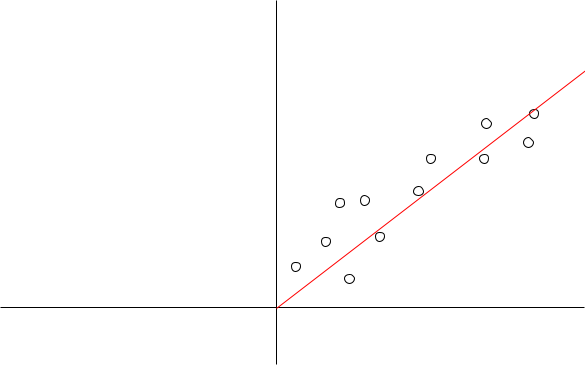
\includegraphics[width=0.3\linewidth]{../common/00_introduction/00_resources/00_approximation.png}
    \end{center}
    \caption{Annäherung an Datenpunkte über lineare Funktion}
    \label{fig:05_approximation}
\end{figure}